% !TeX root = ../tjuthesis-example.tex

\section{文档格式 Document Style}

\subsection{页面格式}

\subsubsection{装订线}

\begin{figure}
    \centering
    
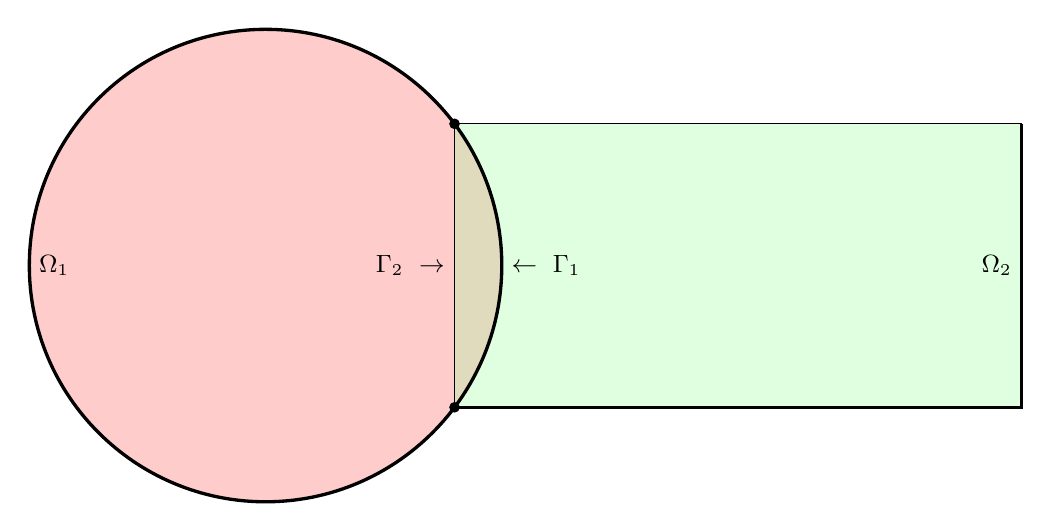
\begin{tikzpicture}[scale=0.6]%[transform canvas={scale=0.6}]
    \filldraw[fill=red,draw=black,fill opacity = 0.2](0,0) circle (5);
    \filldraw[fill=green!40!white, draw=black,fill opacity=0.3] (4,-3) rectangle (16,3);
    %\draw [white,very thin] (4,-3) -- (4,3);
    \draw[very thick] (0,0) circle (5);
    \draw[very thick] (4,-3) -- (16,-3) -- (16,3) ;
    \filldraw[fill=black](4,3) circle [radius = 0.1];
    \filldraw[fill=black](4,-3) circle [radius = 0.1];
    \draw (-5,0) node[anchor=west]{\fontsize{9bp}{10pt}\selectfont $\Omega_1$};
    \draw (4,0) node[anchor=east]{\fontsize{9bp}{10pt}\selectfont $\Gamma_2\  \rightarrow$};
    \draw (5,0) node[anchor=west]{\fontsize{9bp}{10pt}\selectfont $\leftarrow\  \Gamma_1$};
    \draw (16,0) node[anchor=east]{\fontsize{9bp}{10pt}\selectfont $\Omega_2$};
\end{tikzpicture}
\caption{\fontsize{9bp}{18bp}\selectfont Schwarz交替法示意图} \label{fig:schwarzalter}
\end{figure}

装订线由 ``装订线" 三字与unicode字符 U+250A ``┊" 构成, 其中汉字两两之间间隔五个 ``┊" 字符, 而汉字外侧还有十三个 ``┊" 字符. 经过测量, 我们发现装订线整体距离页上边框约为5.89厘米, 距离页下边框约5.02厘米, 而装订线水平中心距离页左边框约1.88厘米, 装订线的行间距约为0.48厘米.

旧版本中我们采用 \pckg{fancybox} 进行装订线的排版. 根据文档我们知道参数中默认页面上有1英寸的边缘, 经过测量我们发现页面左边的边缘约为2.74厘米, 于是我们可以采用
\begin{verbatim}
  \fancyput(-0.86cm,-12.745cm){<gutter-characters>}
\end{verbatim}
的方法来绘制装订线. 不过用宏 \verb|\fancyput| 来绘制装订线会与 verbatim 之类的环境有冲突, 比如我们已经观察到多页的代码会导致装订线有奇怪的表现, 虽然可以通过一些技巧来解决, 但是我们仍有些不满意.

新版本中我们采用了 2020-10-01 版本的 {\LaTeX} 所提供的新特性, 用 \pckg{lthooks} 宏包为每一页在合适的位置画上装订线. 因为绘制装订线的命令变为了 \verb|\put|, 并且我们要支持双页输出, 所以我们需要进行重新测量, 结果为奇数页的参数应为 1.69 厘米与 -15.20 厘米, 而偶数页的参数应为 19.12 厘米与 -15.20 厘米.

\subsubsection{几何与页眉页脚}

经过测量, 我们发现页眉线距离页上边框约为1.33英寸, 距离页左边框约为1.36英寸, 距离页右边框约为0.74英寸, 页脚线距离页下边框约为0.80英寸, 于是经过计算与调整, 我们得到了在 \pckg{geometry} 宏包中应提供的几何数据. 这里我们偷懒了, 没有按照推荐选用 \verb|includeall| 选项, 在今后有必要的话我们可能会进行修复. 此外, 由于我们需要在页眉中放置同济大学的图标, 因此设置了 \verb|headheight = 45pt|. \emph{这里要注意的是, 用页眉线与页脚线测出来的左右页边距不一致, 页眉线与页脚线会往两侧的页边中探出约 0.02 英寸的距离, 因此我们需要比刚才设置的更大的页边距, 并扩大页眉与页脚的宽度.}

页眉页脚我们采用 \pckg{fancyhdr} 进行配置, 页眉页脚中出现的文字及数字均为小四大小, 并且都是宋体字体. 关于页眉, 注意到 ``毕业设计(论文)" 要比页眉线高出一些, 经测量字的顶端距离页眉线约有0.38英寸, 因此我们需要将这几个字用 \verb|\raisebox| 宏抬升0.15英寸左右. 关于页脚, 要注意摘要和目录页是用大写罗马数字编号, 并且需要采用 \verb|\raisebox| 下沉0.02英寸左右, 而正文用阿拉伯数字从一开始重新编号, 并且 ``共\ 页" 与 ``第\ 页" 内部文本与数字的间距为一个汉字宽度, 而它们之间的间距为一点五个汉字宽度. 还要注意的是需要用 \verb|\fancyhfoffset| 宏扩大页眉与页脚的宽度.

\subsection{摘要页}

摘要页包含标题, 摘要以及关键词. 我们先来整理一下手册对摘要页的要求. 手册中第十七页的撰写规范中提到:
\begin{quote}
  课题名称应该简明, 突出主题. 如字数太多, 可分列成主标题和副标题. 字体, 字号详见附件.
  论文内容摘要主要是对撰写过程中实践, 实验, 研究的内容, 方法和得到的主要结果的完整概括, 中文字数一般为300字左右, 并应有相应的英译文.
  设计总说明主要阐述本设计的基础条件, 技术要求, 基本数据, 效果分析 (经济, 社会, 人文等方面) 及简要结论, 中文字数一般为1500字左右及300字左右的英文摘要. 个别无设计说明书的专业, 也应有300字左右的英文设计简介.
  关键词一般3--5个为宜. 字体, 字号参见附件.
\end{quote}
手册第四十四页的打印格式及要求说明中提到:
\begin{quote}
  标题栏居中书写, 黑体, 小二号加粗 (副标题为三号).
\end{quote}
手册第四十五页的参考例文中对中文摘要页有如下要求:
\begin{quote}
  课题名称: 小二号, 黑体, 加粗, 居中, 行距18磅, 段前0.5行, 段后0.5行. 上下各空一行.
  ``摘要" 二字: 四号, 黑体, 居中. 行距18磅. 段前0.5行, 段后0.5行.
  摘要正文300字左右, 五号宋体, 首行缩进2个汉字符. 行距18磅.
  摘要与关键词之间空一行.
  ``关键词" 三字及冒号: 五号宋体, 加粗.
  关键词3--5个, 五号宋体. 逗号分开, 最后一个关键词后面无标点符号.
\end{quote}
手册第四十六页的参考例文中对英文摘要页有如下要求:
\begin{quote}
  英文课题名称: 换页. 小二号, Times New Roman, 加粗, 居中, 行距18磅, 段前0.5行, 段后0.5行, 上下各空一行.
  ``ABSTRACT" 一词: 四号 Times New Roman 居中, 段前0.5行, 段后0.5行. 行距18磅.
  摘要正文: 五号 Times New Roman, 首行缩进2个汉字符, 行距18磅.
  摘要与关键词之间空一行.
  ``Key words" 两词及冒号: 五号 Times New Roman, 加粗.
  关键词: 五号 Times New Roman, 各关键词之间逗号分开, 逗号后加一空格. 行距18磅.
\end{quote}

我们提供了 \verb|abstract| 环境和 \verb|abstract*| 环境来进行中英文摘要的排版. 环境的参数是以逗号分割 (可以加空格) 的关键词列表. 在摘要页的排版中, 我们遇到了一系列 Word 中的术语. 经过研究, 我们发现 Word 中所谓一 ``行" 的高度约为小五号字体大小 (9磅) 的1.2倍, 需要注意的是 ``空一行" 之后我们仍需要添加行距所带来的垂直空白.

中文摘要页中, ``摘要" 二字间距为半个汉字宽度, 因此我们用 \verb|\hspace*{0.5\ccwd}| 来添加这段水平空白. 关键词中我们尊重例文而采用中文标点符号. 标题和 ``关键词" 是加粗的, 这里我们需要用到 \pckg{fontspec} 宏包中的 \verb|FakeBold| 特性, 我们设置了 \verb|EmboldenFactor = 4|, 这与例文的效果相类似. \emph{似乎中文摘要页中的空格之类的本应该用西文字体的符号也都采用了中文字体, 我们并未模仿这一行为.}

英文摘要页中, 参考例文中有两处排版问题. 一是 ``ABSTRACT" 一词例文的注记中未要求加粗, 但是例文中加粗了; 二是 ``Key words" 一词后的冒号例文中采用了宋体的全角冒号, 这似乎不合适. \emph{因此我们改正了这两处排版问题, 使 ``ABSTRACT" 变为不加粗的 Times New Roman 字体, 而将 ``Key words" 后的中文全角冒号改为英文的半角冒号及一个空格.}

\subsection{目录}

我们先来整理一下手册对目录的要求. 手册中第十七页的撰写规范中提到:
\begin{quote}
  目录按照三级标题编写 (即: 1 \dots\dots, 1.1 \dots\dots, 1.1.1 \dots\dots), 要求标题层次清晰. 目录中的标题应与正文中的标题一致, 附录也应依次列入目录.
\end{quote}
手册第四十六页的参考例文中对英文摘要页有如下要求:
\begin{quote}
  ``目录" 二字: 换页, 上下各空一行; 四号黑体居中, 目录2字中间空1格, 段前0.5行, 段后0.5行. 行距18磅.
  目录内容: 五号宋体 (英文 Times New Roman), 单倍行距.
\end{quote}

我们采用 \pckg{tocloft} 宏包进行目录页的排版, 并应用 \verb|titles| 选项用自带的 \verb|\section| 宏来创建目录的标题. 需要注意的是目录下需要空一行, 因此我们给 \verb|\tableofcontents| 宏打了补丁, 临时修改了章标题下的垂直间距, 这里与标题页相同依然要注意手动添加行间距所造成的垂直间距. 目录正文中, 我们需要注意各级标题的编号所占的宽度以及它们的缩进. 经过测量, 我们发现编号所占的宽度分别为 1.5, 2 和 2.75 个汉字宽度, 而编号的缩进分别为 0, 1.25 和 4.5 个汉字宽度. 为了保证不在标题名称后面很近的地方就有一个点, 所以我们在标题后面添加了 0.125 个汉字宽度的空白. 关于页码我们将页码宽度设为了 0.5 个汉字宽度并采用了左对齐, 这样子的话似乎很丑, 不过前九页的页码会与参考例文相同. 值得注意的是似乎我们对 \verb|\@tocrmarg| 宏的设置失效了.

\subsection{章节标题 Titles}

% 示例中说一级标题应换页. 17级应数专业的示例中, 一级标题为小三加粗 (中文字为黑体不加粗, 下同), 二级标题与三级标题均为五号加粗, 序号与标题之间的空格偏大, 应该为两个中文字符 (即 \verb|2\ccwd| ) 的长度.

我们有空的时候再抄章节标题的要求吧. 要注意一级标题换页空一行, 各级标题段前一行段后一行行距18磅, 标题的字体为黑体和Times New Roman. \emph{还要注意的是参考例文中一级标题序号和标题名之间空了一个汉字宽度的空格, 而其余标题的标题序号和标题名之间只空了半个汉字宽度的空格.}

\subsubsection{第三级标题 Subsubsection}

第三级标题应空两格再写序号.

\zhlipsum[1]

\subsection{参考文献}

我们这里所说的是参考文献表的排版, 至于如何引用文献, 请参考\ref{sec:exm-bib}. 我们先来整理一下手册对谢辞的要求. 手册第二十页的撰写规范中提到:
\begin{quote}
  主要参考文献要求 10 篇以上, 其中外文文献 2 篇以上 (指导教师认定为特殊类型的论文, 可以不列外文参考文献).  参考文献必须是公开出版, 发表的 (含网上下载) 著作或者期刊 (论文), 统一放在文后, 并按文中出现的先后顺序, 用阿拉伯数字进行自然编号, 序码加方括号.

  依据中华人民共和过国家标准 GB/T 7714-2015\ldots\ldots\footnote{参考文献著录规则我们就不在这里抄写了.}

  著作方式相同的责任者不超过 3 个时, 全部照录, 超过 3 个时, 著录前 3 个责任者, 其后加 ``, 等" 或与之相对应的词 (英文为 ``,et al."\footnote{原文中为英文逗号, 并且之后没有空格. 在国标中采用的是中文全角的逗号. 而我们目前采用的是英文逗号, 并且之后有一个空格.})
\end{quote}
手册第四十四页的打印格式及要求说明中提到:
\begin{quote}
  ``参考文献" 四字: 居中书写, 黑体, 四号.
  内容: 宋体, 五号.
  参考文按文章中出现的先后, 用方括号阿拉伯数字编号排序 [1] [2] [3] [4] \dots\dots
\end{quote}
手册第五十四页的参考例文中提到:
\begin{quote}
  所有引用的期刊需写出完整刊名. 按论文中参考文献出现的次序, 用阿拉伯数字自然编号, 序码加方括号, 顶格书写.
  参考文献内容: 五号, 宋体 (英文 Times New Roman), 行距 18 磅, 段前0行, 段后0行.
  参考文献不少于10篇, 其中外文文献不少于2篇 (这是最低要求, 各学院可以根据本学院情况制定数量要求).

  注: 期刊若只有期, 没有卷, 则可以省略卷号. 若只有卷, 没有 (或不分) 期, 则可以省略期号.\footnote{我们之后再补上这两条的示例.}
\end{quote}

在参考文献表的排版中, \emph{我们要注意参考例文的 ``参考文献" 四字与页眉的间距与其余一级标题不一致, 我们没有模仿这一行为, 而是保持了除去 ``目录" 的一级标题一直以来的间距.} 我们采用 \pckg{biblatex} 宏包的 \verb|style=biblatex-gb7714-2015| 样式来帮助进行文献著录以及参考文献表的排版, 其中对齐方式采用左对齐, 即 \verb|gbalign=left|, 并将参考文献中序号和内容的间距设为 0.25 个汉字宽度, 虽然这看起来比参考例文中的略小一点 (不到 0.1 个字符宽度), 但是我们不准备调整了.

\subsection{谢辞}

我们先来整理一下手册对谢辞的要求. 手册第二十三页的撰写规范中提到:
\begin{quote}
  谢辞应以简短的文字对在课题研究和论文 (设计) 撰写过程中曾直接给予帮助的人员 (例如指导教师, 答疑教师及其他人员) 表示自己的谢意, 这不仅是一种礼貌, 也是对他人劳动的尊重, 是治学者应有的思想作风.
\end{quote}
手册第四十四页的打印格式及要求说明中提到:
\begin{quote}
  ``谢辞" 二字: 居中, 黑体, 四号.
  内容: 宋体, 五号.
\end{quote}
手册第五十五页的参考例文中提到:
\begin{quote}
  (谢辞) 出自内心, 有感而发. 正文: 五号, 宋体 (英文 Times New Roman), 两端对齐, 段落首行左缩进2个汉字符, 行距18磅, 段前0行, 段后0行.
\end{quote}

谢辞标题与没有编号的一级标题样式相同, ``谢辞" 中间应该有半个汉字宽度的空格.
